\documentclass[a4paper]{article}
\usepackage{geometry}
\usepackage{graphicx}
\usepackage{natbib}
\usepackage{amsmath}
\usepackage{amssymb}
\usepackage{amsthm}
\usepackage{paralist}
\usepackage{epstopdf}
\usepackage{tabularx}
\usepackage{longtable}
\usepackage{multirow}
\usepackage{multicol}
\usepackage[hidelinks]{hyperref}
\usepackage{fancyvrb}
\usepackage{float}
\usepackage{paralist}
\usepackage[svgname]{xcolor}
\usepackage{enumerate}
\usepackage{array}
\usepackage{times}
\usepackage{url}
\usepackage{fancyhdr}
\usepackage{comment}
\usepackage{environ}
\usepackage{times}
\usepackage{textcomp}
\usepackage{caption}
\usepackage{bbm}
\usepackage{enumitem}
\usepackage{algorithm}
\usepackage{algpseudocode}
\usepackage{caption}
\usepackage{subcaption}


\urlstyle{rm}

\setlength\parindent{0pt} % Removes all indentation from paragraphs
\theoremstyle{definition}
\newtheorem{definition}{Definition}[]
\newtheorem{conjecture}{Conjecture}[]
\newtheorem{example}{Example}[]
\newtheorem{theorem}{Theorem}[]
\newtheorem{lemma}{Lemma}
\newtheorem{proposition}{Proposition}
\newtheorem{corollary}{Corollary}

\floatname{algorithm}{Procedure}
\renewcommand{\algorithmicrequire}{\textbf{Input:}}
\renewcommand{\algorithmicensure}{\textbf{Output:}}
\newcommand{\abs}[1]{\lvert#1\rvert}
\newcommand{\norm}[1]{\lVert#1\rVert}
\newcommand{\RR}{\mathbb{R}}
\newcommand{\CC}{\mathbb{C}}
\newcommand{\Nat}{\mathbb{N}}
\newcommand{\br}[1]{\{#1\}}
\DeclareMathOperator*{\argmin}{arg\,min}
\DeclareMathOperator*{\argmax}{arg\,max}
\renewcommand{\qedsymbol}{$\blacksquare$}

\definecolor{dkgreen}{rgb}{0,0.6,0}
\definecolor{gray}{rgb}{0.5,0.5,0.5}
\definecolor{mauve}{rgb}{0.58,0,0.82}

\newcommand{\Var}{\mathrm{Var}}
\newcommand{\Cov}{\mathrm{Cov}}

\newcommand{\vc}[1]{\boldsymbol{#1}}
\newcommand{\xv}{\vc{x}}
\newcommand{\Sigmav}{\vc{\Sigma}}
\newcommand{\alphav}{\vc{\alpha}}
\newcommand{\muv}{\vc{\mu}}

\newcommand{\red}[1]{\textcolor{red}{#1}}

\def\x{\mathbf x}
\def\y{\mathbf y}
\def\w{\mathbf w}
\def\v{\mathbf v}
\def\E{\mathbb E}
\def\V{\mathbb V}
\def\ind{\mathbbm 1}

% TO SHOW SOLUTIONS, include following (else comment out):
\newenvironment{soln}{
	\leavevmode\color{blue}\ignorespaces
}{}

\hypersetup{
	%    colorlinks,
	linkcolor={red!50!black},
	citecolor={blue!50!black},
	urlcolor={blue!80!black}
}

\geometry{
	top=1in,            % <-- you want to adjust this
	inner=1in,
	outer=1in,
	bottom=1in,
	headheight=3em,       % <-- and this
	headsep=2em,          % <-- and this
	footskip=3em,
}


\pagestyle{fancyplain}
\lhead{\fancyplain{}{Homework 6}}
\rhead{\fancyplain{}{CS 760 Machine Learning}}
\cfoot{\thepage}

\title{\textsc{Homework 6}} % Title

%%% NOTE:  Replace 'NAME HERE' etc., and delete any "\red{}" wrappers (so it won't show up as red)

\author{
	Harry Zhang\\
	hzhang699@wisc.edu\\
	GitHub Repo: 
} 

\date{}

\begin{document}
	
	\maketitle 
	
        \textbf{Instructions:}
        Use this latex file as a template to develop your homework. Submit your homework on time as a single pdf file. Please wrap your code and upload to a public GitHub repo, then attach the link below the instructions so that we can access it. Answers to the questions that are not within the pdf are not accepted. This includes external links or answers attached to the code implementation. Late submissions may not be accepted. You can choose any programming language (i.e. python, R, or MATLAB). Please check Piazza for updates about the homework. It is ok to share the results of the experiments and compare them with each other.
        \vspace{0.1in}
	
	\section{Implementation: GAN (50 pts)}
	In this part, you are expected to implement GAN with MNIST dataset. We have provided a base jupyter notebook (gan-base.ipynb) for you to start with, which provides a model setup and training configurations to train GAN with MNIST dataset.
	
	\begin{enumerate} [label=(\alph*)]
		\item Implement training loop and report learning curves and generated images in epoch 1, 50, 100. Note that drawing learning curves and visualization of images are already implemented in provided jupyter notebook. \hfill (20 pts)
		
		\begin{algorithm}
			\caption{Training GAN, modified from \cite{goodfellow2014generative}}\label{alg:GAN}
			\begin{algorithmic}
				\Require $m$: real data batch size, $n_{z}$: fake data batch size
				\Ensure Discriminator $D$, Generator $G$
				
				\For{number of training iterations}
				
				\State{$\#$ Training discriminator}
				\State{Sample minibatch of $n_{z}$ noise samples $\{z^{(1)}, z^{(2)}, \cdots, z^{(n_{z})}\}$ from noise prior $p_{g}(z)$}
				\State{Sample minibatch of $\{x^{(1)}, x^{(2)}, \cdots, x^{(m)}\}$}
				\State{Update the discriminator by ascending its stochastic  gradient:
					$$\nabla_{\theta_{d}} \big ( \cfrac{1}{m}  \sum_{i=1}^{m}  \log D(x^{(i)})  + \cfrac{1}{n_{z}} \sum_{i=1}^{n_{z}}  \log (1-D(G(z^{(i)})))\big )$$
				}
				
				\State{$\#$ Training generator}
				\State{Sample minibatch of $n_{z}$ noise samples $\{z^{(1)}, z^{(2)}, \cdots, z^{(n_{z})}\}$ from noise prior $p_{g}(z)$}
				\State{Update the generator  by ascending its stochastic  gradient:
					$$\nabla_{\theta_{g}}  \cfrac{1}{n_{z}} \sum_{i=1}^{n_{z}}  \log D(G(z^{(i)}))\big )$$
				}
				\EndFor
				
				\State{$\#$ The gradient-based updates can use any standard gradient-based learning rule. In the base code, we are using Adam optimizer \citep{kingma2014adam}}
			\end{algorithmic}
		\end{algorithm}
		
		% Expected results are as follows.
		
		\begin{figure}[H]
			\centering
			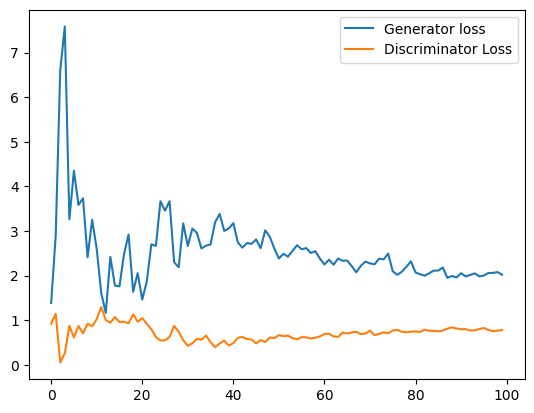
\includegraphics[width=0.7\textwidth]{gan_q1_loss.png}
			\caption{Learning curve}
			\label{fig:gan_q1_loss}
		\end{figure}
		
		\begin{figure}[H]
			\centering
			\begin{subfigure}[b]{0.3\textwidth}
				\centering
				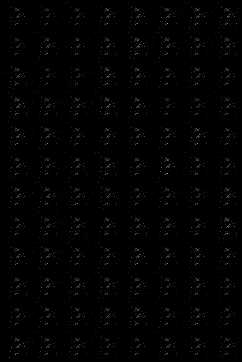
\includegraphics[width=\textwidth]{gan_q1a_epoch1.png}
				\caption{epoch 1}
			\end{subfigure}
			\hfill
			\begin{subfigure}[b]{0.3\textwidth}
				\centering
				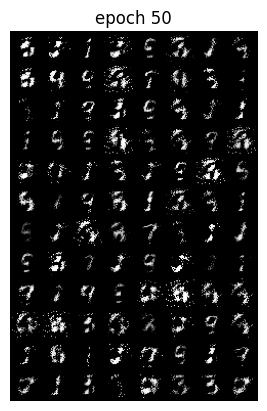
\includegraphics[width=\textwidth]{gan_q1a_epoch50.png}
				\caption{epoch 50}
			\end{subfigure}
			\hfill
			\begin{subfigure}[b]{0.3\textwidth}
				\centering
				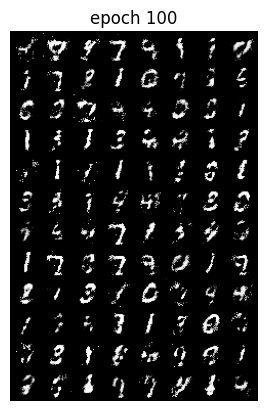
\includegraphics[width=\textwidth]{gan_q1a_epoch100.png}
				\caption{epoch 100}
			\end{subfigure}
			\caption{Generated images by $G$}
			\label{fig:three graphs}
		\end{figure}
		
		
		\begin{soln} \\
		For images see Fig.~\ref{fig:three graphs}; For learning curve see Fig.~\ref{fig:gan_q1_loss} \end{soln}
		
		
		
		\item Replace the generator update rule as the original one in the slide,\\
		``Update the generator by descending its stochastic gradient:
		
		$$\nabla_{\theta_{g}}  \cfrac{1}{n_{z}}  \sum_{i=1}^{n_{z}}\log (1-D(G(z^{(i)})))\big )$$
		"
		, and report learning curves and generated images in epoch 1, 50, 100. Compare the result with (a). Note that it may not work. If training does not work, explain why it doesn't work. \\
        You may find this helpful: https://jonathan-hui.medium.com/gan-what-is-wrong-with-the-gan-cost-function-6f594162ce01
		\hfill (10 pts)
		
		\begin{figure}[H]
			\centering
			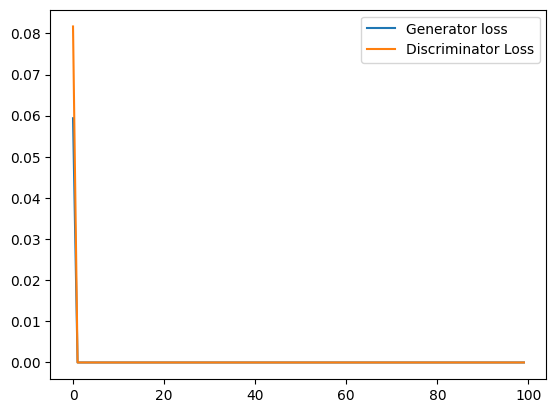
\includegraphics[width=0.7\textwidth]{gan_q1b_loss.png}
			\caption{Learning curve}
			\label{fig:gan_q1b_loss}
		\end{figure}
		
		\begin{figure}[H]
			\centering
			\begin{subfigure}[b]{0.3\textwidth}
				\centering
				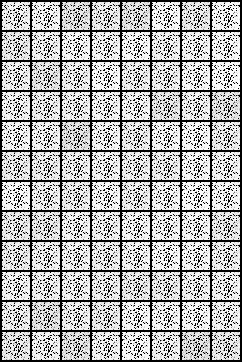
\includegraphics[width=\textwidth]{gan_q1b_epoch1.png}
				\caption{epoch 1}
			\end{subfigure}
			\hfill
			\begin{subfigure}[b]{0.3\textwidth}
				\centering
				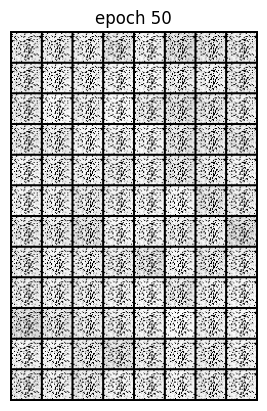
\includegraphics[width=\textwidth]{gan_q1b_epoch50.png}
				\caption{epoch 50}
			\end{subfigure}
			\hfill
			\begin{subfigure}[b]{0.3\textwidth}
				\centering
				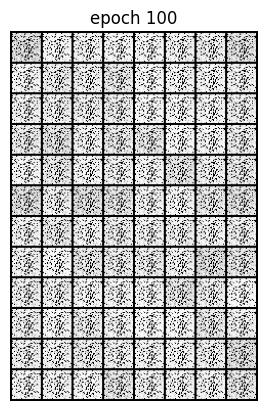
\includegraphics[width=\textwidth]{gan_q1b_epoch100.png}
				\caption{epoch 100}
			\end{subfigure}
			\caption{Generated images by $G$}
			\label{fig:threegraphs_q1b}
		\end{figure}
		
		
		\begin{soln} \\
		For images see Fig.~\ref{fig:threegraphs_q1b}; For learning curve see Fig.~\ref{fig:gan_q1b_loss} \\
		The training does not work. The reason is that the gradient of the generator is 0 when discriminator becomes optimal D*(based on link). In this case, the generator cannot learn anything. 
		\end{soln}

		\item Except the method that we used in (a), how can we improve training for GAN? Implement that and report your setup, learning curves, and generated images in epoch 1, 50, 100.
        This question is an open-ended question and you can choose whichever method you want.
		\hfill (20 pts)
		

		\begin{figure}[H]
			\centering
			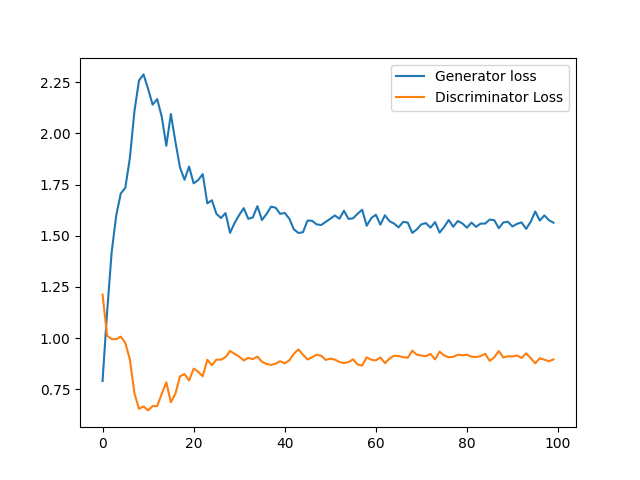
\includegraphics[width=0.6\textwidth]{gan_q1c_loss.png}
			\caption{Learning curve}
			\label{fig:gan_q1c_loss}
		\end{figure}
		
		\begin{figure}[H]
			\centering
			\begin{subfigure}[b]{0.28\textwidth}
				\centering
				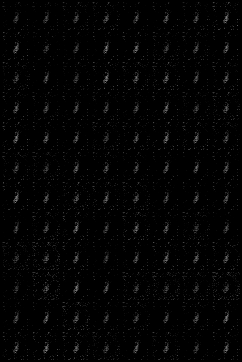
\includegraphics[width=\textwidth]{gen_img1.png}
				\caption{epoch 1}
			\end{subfigure}
			\hfill
			\begin{subfigure}[b]{0.28\textwidth}
				\centering
				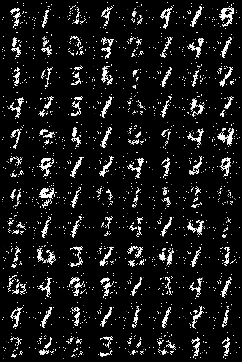
\includegraphics[width=\textwidth]{gen_img20.png}
				\caption{epoch 20}
			\end{subfigure}
			\hfill
			\begin{subfigure}[b]{0.28\textwidth}
				\centering
				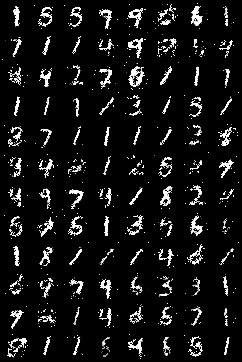
\includegraphics[width=\textwidth]{gen_img50.png}
				\caption{epoch 50}
			\end{subfigure}
			\hfill
			\begin{subfigure}[b]{0.28\textwidth}
				\centering
				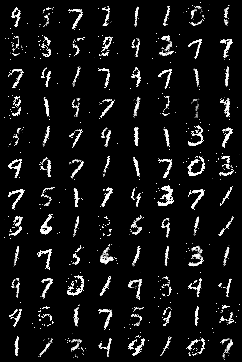
\includegraphics[width=\textwidth]{gen_img80.png}
				\caption{epoch 80}
			\end{subfigure}
			\hfill
			\begin{subfigure}[b]{0.28\textwidth}
				\centering
				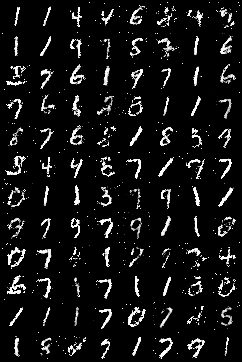
\includegraphics[width=\textwidth]{gen_img100.png}
				\caption{epoch 100}
			\end{subfigure}
			\caption{Generated images by $G$}
			\label{fig:threegraphs_q1c}
		\end{figure}


		\begin{soln}  \\
		I modified the Adam optimizer to ``RMSprop'' optimizer. The learning rate is 0.0002. Looks like this solver gives faster converges rate and from earlier stage of training, we can already see the figures. And also the result after 30 epoches are getting constantly stable.\\
		\end{soln}
		
	\end{enumerate}

\section{Directed Graphical Model [25 points]}
Consider the directed graphical model (aka Bayesian network) in Figure~\ref{fig:bn}.
\begin{figure}[H]
    \centering
    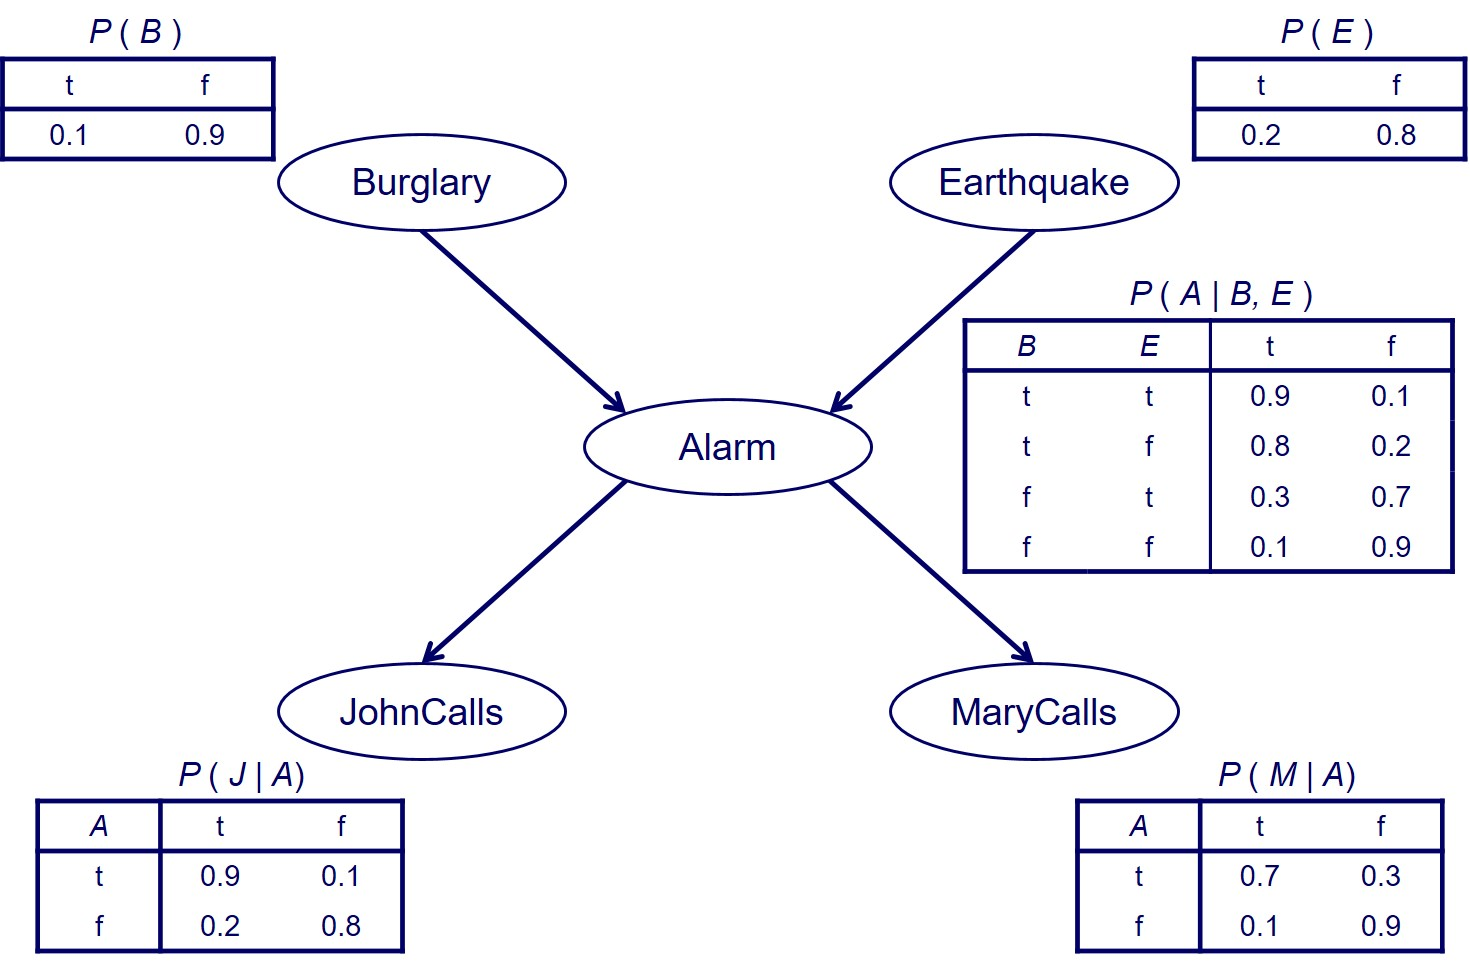
\includegraphics[width=0.8\textwidth]{BN.jpeg}
    \caption{A Bayesian Network example.}
    \label{fig:bn}
\end{figure}
Compute $P(B=t \mid E=f,J=t,M=t)$ and $P(B=t \mid E=t,J=t,M=t)$. (10 points for each) These are the conditional probabilities of a burglar in your house (yikes!) when both of your neighbors John and Mary call you and say they hear an alarm in your house, but without or with an earthquake also going on in that area (what a busy day), respectively.

\begin{soln}
\\
(1)
\begin{align*}
	P&(B=t \mid E=f, J=t, M=t) \\
	&= \frac{P(B=t, E=f, J=t, M=t)}{P(E=f, J=t, M=t)} \\
	&= \frac{P(B=t, E=f, J=t, M=t)}{P(B=t, E=f, J=t, M=t) + P(B=f, E=f, J=t, M=t)} \\
\end{align*}
\begin{align*}
P&(B=t, E=f, J=t, M=t) \\
&= \sum_{a \in A, \neg A} P(B) P(\neg E) P(a \mid B, \neg E) P(J \mid a) P(M \mid a) \\
&= 0.1 \times 0.8 \times 0.8 \times 0.9 \times 0.7 + 0.1 \times 0.8 \times 0.2 \times 0.2 \times 0.1 \\
&= 0.04064
\end{align*}
\begin{align*}
P&(B=f, E=f, J=t, M=t) \\
&= \sum_{a \in A, \neg A} P(\neg B) P(\neg E) P(a \mid \neg B, \neg E) P(J \mid a) P(M \mid a) \\
&= 0.9 \times 0.8 \times 0.1 \times 0.9 \times 0.7 + 0.9 \times 0.8 \times 0.9 \times 0.2 \times 0.1 \\
&= 0.05832
\end{align*}
\begin{align*}
	P&(B=t \mid E=f, J=t, M=t) \\
	&= \frac{P(B=t, E=f, J=t, M=t)}{P(B=t, E=f, J=t, M=t) + P(B=f, E=f, J=t, M=t)} \\
	&= \frac{0.04064}{0.04064 + 0.05832} \\&= 0.41067
\end{align*}

(2): By the same method, we can get:
\begin{align*}
	P&(B=t \mid E=t, J=t, M=t) \\
	&= \frac{P(B=t, E=t, J=t, M=t)}{P(B=t, E=t, J=t, M=t) + P(B=f, E=t, J=t, M=t)} \\
	&= \frac{P(B,E,J,M)}{P(B,E,J,M) + P(\neg B,E,J,M)} \\
\end{align*}

\begin{align*}
P&(B,E,J,M) = \sum_{a \in A, \neg A} P(B) P(E) P(a \mid B, E) P(J \mid a) P(M \mid a)\\
&= 0.1 \times 0.2 \times 0.9 \times 0.9 \times 0.7 + 0.1 \times 0.2 \times 0.1 \times 0.2 \times 0.1 \\
&= 0.01138
\end{align*}

\begin{align*}
P&(\neg B,E,J,M) = \sum_{a \in A, \neg A} P(\neg B) P(E) P(a \mid \neg B, E) P(J \mid a) P(M \mid a)\\
&= 0.9 \times 0.2 \times 0.3 \times 0.9 \times 0.7 + 0.9 \times 0.2 \times 0.7 \times 0.2 \times 0.1 \\
&= 0.03654
\end{align*}

\begin{align*}
	P&(B=t \mid E=t, J=t, M=t) \\
	&= \frac{P(B,E,J,M)}{P(B,E,J,M) + P(\neg B,E,J,M)} \\
	&= \frac{0.01138}{0.01138 + 0.03654} \\&= 0.237
\end{align*}

\end{soln}


\section{Chow-Liu Algorithm [25 pts]}
Suppose we wish to construct a directed graphical model for 3 features $X$, $Y$, and $Z$ using the Chow-Liu algorithm. We are given data from 100 independent experiments where each feature is binary and takes value $T$ or $F$. Below is a table summarizing the observations of the experiment:

\begin{table}[H]
        \centering
                \begin{tabular}{cccc}
                           $X$ & $Y$ & $Z$ & Count \\
                                \hline
                                T & T & T & 36 \\
                                \hline
                                T & T & F & 4 \\
                                \hline
                                T & F & T & 2 \\
                                \hline
                                T & F & F & 8 \\
                                \hline
                                F & T & T & 9 \\
                                \hline
                                F & T & F & 1 \\
                                \hline
                                F & F & T & 8 \\
                                \hline
                                F & F & F & 32 \\
                                \hline
                \end{tabular}
\end{table}

\begin{enumerate}
	\item Compute the mutual information $I(X, Y)$ based on the frequencies observed in the data. (5 pts)
	\begin{soln}
		\begin{align*}
			I(X, Y) &= \sum_{x \in X, \neg X, y \in Y,\neg X} P(x, y) \log \frac{P(x, y)}{P(x) P(y)} \\
			&= 0.4 \log \frac{0.4}{0.5 \times 0.5} + 0.1 \log \frac{0.1}{0.5 \times 0.5} + 0.1 \log \frac{0.1}{0.5 \times 0.5} + 0.4 \log \frac{0.4}{0.5 \times 0.5} \\
			&= 0.278
		\end{align*}
	\end{soln}
	\item Compute the mutual information $I(X, Z)$ based on the frequencies observed in the data. (5 pts)
	\begin{soln}
		\begin{align*}
			I(X, Z) &= \sum_{x \in X, \neg X, z \in Z,\neg Z} P(x, z) \log \frac{P(x, z)}{P(x) P(z)} \\
			&= 0.38 \log \frac{0.38}{0.55 \times 0.5} + 0.12 \log \frac{0.12}{0.45 \times 0.5} + 0.17 \log \frac{0.17}{0.55 \times 0.5} + 0.33 \log \frac{0.33}{0.5 \times 0.45} \\
			&= 0.1328
		\end{align*}
	\end{soln}
	\item Compute the mutual information $I(Z, Y)$ based on the frequencies observed in the data. (5 pts)
	\begin{soln}
		\begin{align*}
			I(Y, Z) &= \sum_{y \in Y, \neg Y, z \in Z,\neg Z} P(y, z) \log \frac{P(y, z)}{P(y) P(z)} \\
			&= 0.45 \log \frac{0.45}{0.55 \times 0.5} + 0.05 \log \frac{0.05}{0.45 \times 0.5} + 0.1 \log \frac{0.1}{0.55 \times 0.5} + 0.4 \log \frac{0.4}{0.5 \times 0.45} \\
			&= 0.3973
		\end{align*}
	\end{soln}

	\item Which undirected edges will be selected by the Chow-Liu algorithm as the maximum spanning tree? (5 pts)
	\begin{soln}
		Since $I(Y, Z) > I(X, Y) > I(X, Z)$, the edges $(Y,Z)$ and $(X,Y)$ will be selected, and we will not select $(X,Z)$ because adding $(X,Z)$ will form a cycle.
	\end{soln}
	\item Root your tree at node $X$, assign directions to the selected edges. (5 pts)
	\begin{soln}
		\begin{figure}[H]
			\centering
			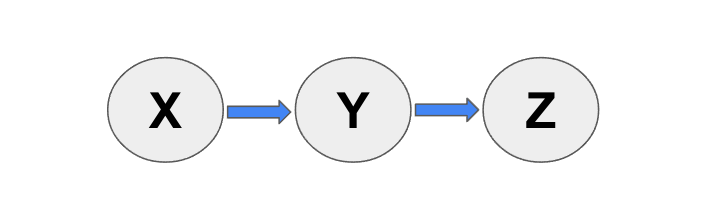
\includegraphics[width=0.5\textwidth]{TREE.png}
			\caption{Directed Graphical Model}
			\label{fig:diagram}
		\end{figure}
		See Figure \ref{fig:diagram}.
	\end{soln}
\end{enumerate}

	\bibliography{hw6}
	\bibliographystyle{apalike}
\end{document}
